\section{对此前模型的分析}
% USR-DU的DSN部分负责由高分辨率图像生成对应的拟真低分辨率图像。图中展示了DSN对DIV2K\parencite{timofte2017ntire}和RealSR-Canon数据集中图像生成低分辨率图像的效果。其中,针对模糊性较低的DIV2K数据集,生成的低分辨率图像与真实的低分辨率图像较为相似,而对于模糊性较高的RealSR-Canon数据集,DSN生成的低分辨率图像会显得过于清晰,同时二者还存在色差的问题。对于造成这种现象的原因,我们推测是由DSN部分直接使用高分辨率图像的双三次下采样结果作为参考图像所导致的,如图虚线部分。由于DSN使用data loss和perceptual loss来对网络进行优化,这使得生成的低分辨率图像在一定程度上近似于无模糊的图像,从而远离了真实的低分辨率图像。因此,为了对此模型进一步优化,提高其泛化能力,我们提出了改进模型UBSR-DU,即基于不确定性学习的无监督的模糊真实世界图像超分辨率(Unsupervised Blurry real-world image SR with learned Degradation Uncertainty)。

USR-DU的DSN部分负责由高分辨率图像生成对应的拟真低分辨率图像。
\section{基于不确定性学习的无监督的模糊真实世界图像超分辨率}
在无监督的超分辨率模型中,我们需要首先生成拟真的低分辨率图像,再对超分网络进行监督式的训练,而对图像的退化过程进行合理的建模将有助于提升低分辨率图像生成的精度。在本节接下来的内容中,我们将首先给出图像的退化模型,随后由此引出我们提出的改进模型UBSR-DU。
\subsection{图像的退化过程}
真实世界低分辨率图像的退化过程与合成低分辨率图像的退化过程有着显著的差别。合成图像数据集往往假设低分辨率图像由高分辨率图像经高斯模糊和双三次下采样得到,使用公式表示即为:
\begin{equation}
    \mathbi{I}^{LR}=(\vb*{k}_g\otimes \mathbi{I}^{HR})\downarrow_s
\end{equation}
其中,$\mathbi{I}^{LR}$和$\mathbi{I}^{HR}$分别表示低分辨率图像和高分辨率图像,$\vb*{k}_g$表示高斯核,$\otimes$表示卷积操作,$\downarrow_s$表示双三次下采样。

对于真实低分辨率图像,情况要复杂的多,不过,其退化过程往往也可以近似为以下过程:首先使用各向异性高斯核对高分辨率图像进行滤波,再经过双三次下采样,最后加上噪声。使用公式描述即为
\begin{equation}
    \mathbi{I}^{LR}=(\vb*{k}\otimes \mathbi{I}^{HR})\downarrow_s+\mathbi{n}
\end{equation}
其中$\vb*{k}$为未知的各向异性高斯核,$\mathbi{n}$为未知的噪声。是所以认定为各向异性高斯核,是因为\parencite{Gau_1}\parencite{Gau_2}\parencite{Gau_3}\parencite{Gau_4}\parencite{Gau_5}等工作表明,各向异性高斯核先验对超分辨率任务来说是完备的。
%此处引用FKP提到的文章

以上过程假设图像退化时,模糊核是空间不变的,即对每一个像素点,都有完全相同的模糊核,然而在实际情况中,由于物体运动、景深等因素,图像各处的模糊程度往往是不同的,于是就有了空间可变的真实图像退化过程。
\begin{equation}
    \mathbi{I}^{LR}=(\mathbi{K}\mathbi{I}^{HR})\downarrow_s+\mathbi{n}\label{equ:degrade_sv}
\end{equation}
其中$\mathbi{K}$是一个模糊矩阵,其第$i$行对应于$\mathbi{I}^{HR}$第$i$个像素的模糊核,此模糊核亦基于各向异性高斯核先验。
\subsection{提出的方法}

\begin{algorithm}
    \caption{Generate Reference Image $y_{ref}$}
    \label{alg:y_ref}
    \begin{algorithmic}[1]
        \Require Real LR $y_r$, Real HR $x_r$
        \Ensure Reference Image $y_{ref}$
        \State K $\leftarrow $\Call{MANet}{$y_r$}
        \State $x_{e} \leftarrow$ \Call{UNFOLD}{$x_r$}
        \State $y_{e} \leftarrow K \odot x_{e}$
        \State $y_{e} \leftarrow$ \Call{SUM}{$y_{e}$, dim=3}
        \State $y_{ref} \leftarrow$ \Call{FOLD}{$y_{e}$}
    \end{algorithmic}
\end{algorithm}


\noindent\textbf{总体结构}\ \ 在DSN训练过程中,输入的batch中包含两部分数据:真实的高分辨率图像和低分辨率图像,二者是不成对的。如图\ref{fig:UBSR-DU}所示,为了能将低分辨率图像的模糊信息引入到模型中,我们使用合理的模糊核估计模型对真实低分辨率图像进行模糊核估计,并使用估计的模糊核对高分辨率图像进行退化操作,产生模糊的低分辨率图像,作为网络的参考图像,而不是如同USR-DU中直接使用双三次下采样图像作为参考图像。

\begin{figure}[h]
    \centering
    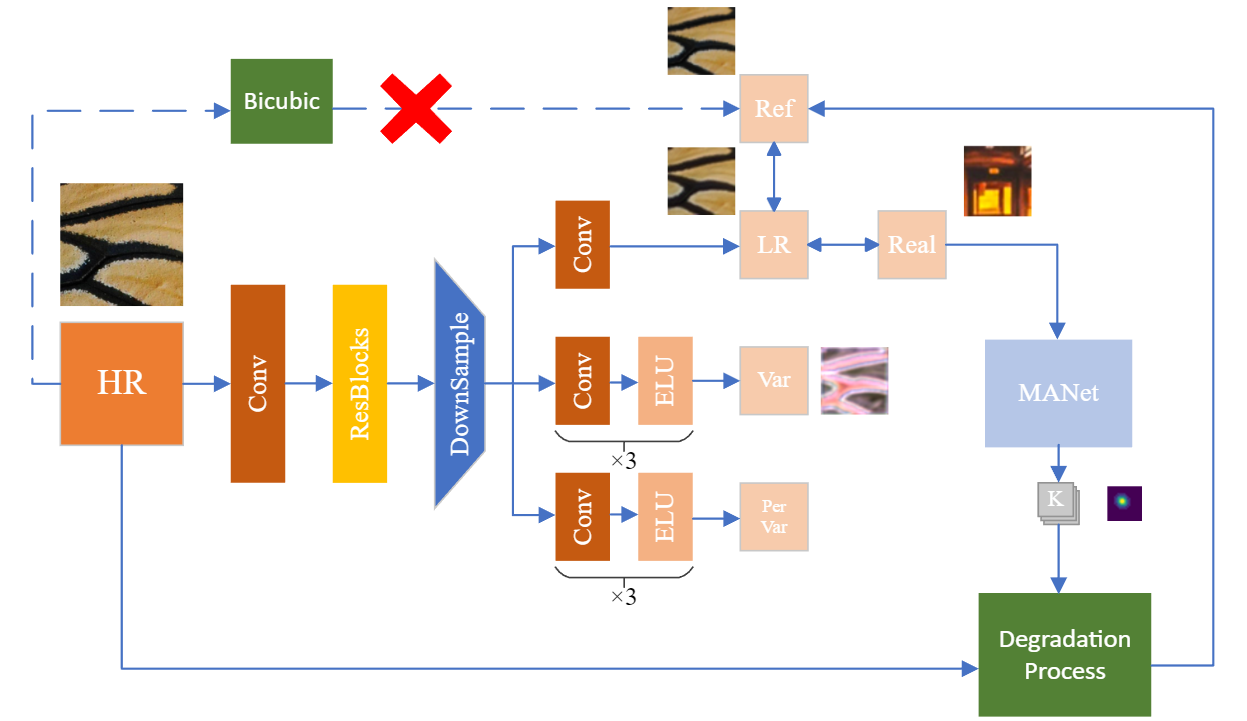
\includegraphics[width=1.0\textwidth]{imgs/UBSR-DU.png}
    \caption{UBSR-DU}
    \label{fig:UBSR-DU}
\end{figure}


\noindent\textbf{模糊核估计}\ \ 目前,已经有许多成熟的低分辨率图像模糊核估计方法,如KULNet、MANet、UFPNet等,其中有空间不变的核估计,也有空间变化的核估计,虽然这些模型都取得了较大的成功,但它们大多不是专门设计用来进行模糊核估计的,而是属于其他任务内部的一个中间过程,而这些任务的优化的目标往往也不包含模糊核估计精度,换言之,其估计的模糊核本身并不一定精准。而在本文中,为了能得到更加真实的参考图像,我们需要一个能够最精准的估计模糊核本身的模型。我们对Canon数据集训练集高分辨率图像进行了随机的各向异性高斯模糊并进行下采样,手工合成了一系列低分辨率图像,其中,模糊核是已知的。我们分别用KULNet、MANet、UFPNet这三种模糊核估计网络对合成的低分辨率网络进行了核估计,估计结果如图所示。可以看到,KULNet对所有图像均估计出了相似的近乎各向同性的高斯核,与实际的模糊核并不相似,而MANet和UFPNet则估计出了与实际更为相似的模糊核,故首先排除了KULNet的后续使用。为了在MANet和UFPNet中选择更为合适的模型,我们统计了二者估计模糊核的PSNR指标,并最终选择了UFPNet作为UBSR-DU的模糊核估计模型。

\noindent\textbf{参考图像的生成}\ \ 参考图像生成是一个复杂的过程,尤其是当模糊核空间可变时,在这种情况下,无法直接通过PyTorch提供的卷积模块进行图像退化,需要自行实现。直观的方法是使用两个嵌套循环对batch中的每张图像的每个像素分别进行模糊,随后对所有图像进行下采样,然而,在实际操作中,这种计算方法受制于Python的性能问题,不能有效地利用已经过彻底优化的CUDA算子,使得训练速度大幅减缓。为了能够更有效率的执行图像退化操作,我们选择了MANet所提供的图像退化方案。如算法\ref{alg:y_ref}所示。首先,由MANet估计出的空间可变模糊核为一个尺寸为$(B,C,H_{x_r}\cdot W_{x_r},H_{ker}\cdot W_{ker})$的多维矩阵,其中,B为batch大小,C为通道数(对于RGB图图像来说,取3),$H_{x_r},W_{x_r}$为真实高分辨率图像的高和宽,$H_{ker},W_{ker}$为模糊核的高和宽。故对输入图像$x_r$执行UNFOLD操作,使得卷积过程中每个需要执行矩阵乘法的$H_{ker}\times W_{ker}$区域(即每一个滑动窗口)展开为列向量,并将每个通道的所有列向量向量组成二维矩阵,最终,也形成尺寸为$(B,C,H_{x_r}\cdot W_{x_r},H_{ker}\cdot W_{ker})$的多维矩阵。两个矩阵按元素相乘,并在模糊核向量维度上求和(相当于卷积中的求和操作),最后对结果执行FOLD操作,将矩阵还原为模糊后的图像,并对此图像进行双三次下采样到与DSN生成图像相同尺寸。通过此方式能够最大化地利用利用已经充分优化过的API,从而提高了图像退化的效率,其缺点在于空间复杂度较高,需要较高的显存支持,但与其降低的大量时间成本相比,此缺点可以忽略不计。

\noindent\textbf{DSN的损失函数}\ \ 如图所示,改进后的DSN会产生四个张量,参考低分辨率图像$y_{ref}$、生成低分辨率图像$y_g$、生成图像的不确定性$\theta$和生成图像的特征不确定性$\sigma$。DSN生成器的损失函数使用上述张量与数据集中的真实低分辨率图像$y_r$计算,分为以下三个部分:

内容损失:约束生成的图像在内容上与高分辨率图图像一致,同时能够学习到真实图像的模糊信息,使用KL散度计算,有
\begin{equation}
    \mathcal{L}_{kl}=\mathbb{E}_{\vb*{y}_g}\{D_{\text{KL}}[L(\vb*{y}_g,\bm{\theta})\|L(\vb*{y}_ref,\mathbi{I})]\}
\end{equation}

感知损失:约束生成的图像在特征域上与高分辨率图像一致,同时能够学习到真实图像的模糊信息,使用KL散度计算,有
\begin{equation}
    \mathcal{L}_{kl\_per}=\mathbb{E}_{\vb*{y}_g}\{D_{\text{KL}}[L(\Phi(\vb*{y}_g),\bm{\theta})\|L(\Phi(\vb*{y}_ref),\mathbi{I})]\}
\end{equation}
其中,$\Phi(\cdot)$为VGG-19\parencite{simonyan2014very}。

对抗性损失:使得DSN能够学到真实低分辨率图像纹理细节信息。此处使用了高通滤波保留图像的高频纹理信息。
\begin{equation}
    \mathcal{L}_{adv}^G=\mathbb{E}_{\vb*{y}_g}[\log(D(F(\vb*{y}_g)))]
\end{equation}
其中F为高通滤波器,D为DSN的判别器。

故总的损失函数为
\begin{equation}
    \mathcal{L}_{DSN} = \alpha_1\mathcal{L}_{kl}+\alpha_2\mathcal{L}_{kl\_per}+\alpha_3\mathcal{L}_{adv}^G
\end{equation}
其中,$\alpha_1,\alpha_1,\alpha_1$为超参数,在本文中,依次取值为100.0,1.0,1.0。

DSN的判别器损失函数与原USR-DU相同。

\subsection{对文字内容重建能力的提升}
RealSR通过调整相机的焦距,提供了真实成对的高低分辨率图像数据集,其低分辨率图像具有较强的模糊性。由于本文主要对USR-DU的DSN部分在模糊性学习上做了改进,故使用200张RealSR-Canon-x4的训练集低分辨率图像作为DSN的训练集低分辨率图像,而使用DIV2K提供的800张训练集高分辨率图像(0001-0800)作为DSN训练集的高分辨率图像。对于SRN部分,与USR-DU不同,本文除了使用DIV2K训练集高分辨率图像以外,另外添加了RealSR-Nikon的训练集高分辨率图像,一起组成SRN的训练集高分辨率图像,并使用训练好的DSN生成对应的低分辨率图像,组成SRN的训练集。这是因为SRN的验证集为RealSR-Canon验证集,其中包含了较多的文字内容,而DIV2K中的文字内容较少,会使得训练出的模型生成的超分辨率图像中文字分辨能力较低。故额外添加了包含较多的文字内容的RealSR-Nikon训练集以增强模型对文字的重建能力。
\section{实验}
\subsection{实验设置}
\noindent\textbf{评价指标}\ \ 由于SRN使用成对数据集进行验证,故我们使用PSNR和SSIM来评价重建出来的超分图像在像素和结构上与真实高分辨率图像的相似性。

\noindent\textbf{实现细节}\ \ 对于DSN和SRN的主体网络部分,均沿用了USR-DU的设计。与USR-DU不同的是,DSN中额外加入了加入了一个参考图像生成模块用于生成更加合理的参考图像,其中包含了模糊核估计部分和图像退化部分,如图所示。在DSN中,我们分别使用$192\times192$和$48\times48$的尺寸裁剪高、低分辨率图像,估计的模糊核尺寸设定为$21\times21$,模型以16为batch大小训练了50000个batch,使用Adam优化器,初始学习率为$5\times10^{-5}$,每10000个batch就将学习率减半。在SRN中,我们分别使用$256\times256$和$64\times64$的尺寸裁剪高、低分辨率图像,模型以16为batch大小训练了100000个batch,使用Adam优化器,学习率恒定为$1\times10^{-4}$。二者训练过程,训练集图像均采取了随机的旋转和翻转。我们的方法基于PyTorch和BasicSR\parencite{basicsr}框架实现,并使用NVIDIA TESLA A100(40GB)GPU进行训练。
\subsection{实验结果}
\noindent\textbf{定量比较}\ \ 表\ref{tab:results}中展示了我们提出的改进模型UBSR-DU在RealSR-Canon数据集上与几种当前最先进模型的表现的对比,其中包括了ZSSR、(使用合成数据集)预训练的ESRGAN、DASR、原模型USR-DU。我们还展示了使用RealSR-Canon训练集部分成对图像进行监督式训练的ESRGAN的表现作为参考。从表中可以看到,我们的改进模型UBSR-DU的表现在RealSR-Canon数据集上超出了所有当前最先进的方法,尤其是相比原始模型USR-DU在PSNR和SSIM这两个指标上分别提高了0.07dB和0.0012。


% 表中展示了UBSR-DU在RealSR-Canon验证集上PSNR和SSIM的表现,可以发现,在这两个指标上,UBSR-DU相对当前最先进的模型均有明显的提升,特别的,PSNR和SSIM比UBSR-DU的表现分别高0.07dB和0.0012,这表明UBSR-DU中所做出的改进对于提升模糊低分辨率图像的超分效果是切实有效的。

\begin{table}[htbp]
    \centering
    \caption{在RealSR-Canon数据集上与当前最先进模型的对比}
    \label{tab:results}
    \begin{tblr}{
        colspec={ccc},
        hline{1,8} = {1pt,solid},
        hline{2,7} = {0.5pt,solid},
        vline{2} = {0.5pt,solid}
    }
         & PSNR$\uparrow$  &  SSIM$\uparrow$ \\
        ZSSR & 26.01 & 0.7485 \\
        P.T. ESRGAN & 26.06 & 0.7542 \\
        DASR & 26.23 & 0.7656 \\ 
        USR-DU & 26.56 & 0.7736 \\
        UBSR-DU(ours) & \textbf{26.63} & \textbf{0.7748} \\Z
        S.T. ESRGAN & 25.68 & 0.7271 \\
    \end{tblr}
\end{table}


\noindent\textbf{感官比较}\ \ 我们在图图图中展示我们的模型和其他当前最先进模型生成的超分图像。其中,图展现了UBSR-DU在文字内容重建方面的优势,图展现了我们的模型对于边缘恢复的能力,图展现了我们的模型对于纹理细节的恢复能力。



% \begin{figure}[htbp]
%     \begin{minipage}{0.33\textwidth}
%         \begin{subfigure}{\textwidth}
%             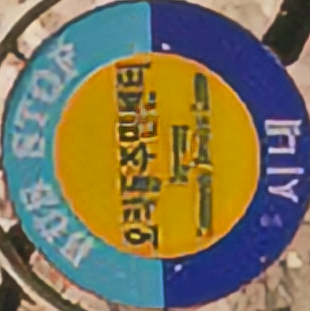
\includegraphics[width=\linewidth]{imgs/DASR_23.83_0.7483_Canon_020.png}
%             \caption{1} 
%         \end{subfigure}
%     \end{minipage}
%     \hfill
%     \begin{minipage}{0.66\textwidth}
%         \begin{subfigure}{0.22\textwidth}
%             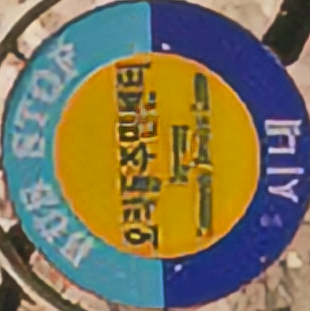
\includegraphics[width=\linewidth]{imgs/DASR_23.83_0.7483_Canon_020.png}
%             \caption{2} 
%         \end{subfigure}
%         \hfill
%         \begin{subfigure}{0.22\textwidth}
%             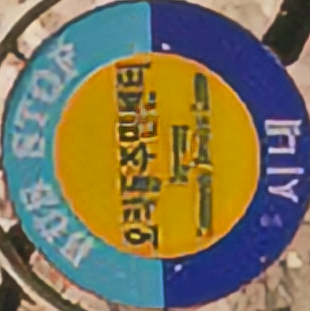
\includegraphics[width=\linewidth]{imgs/DASR_23.83_0.7483_Canon_020.png}
%             \caption{3} 
%         \end{subfigure}
%         \hfill
%         \begin{subfigure}{0.22\textwidth}
%             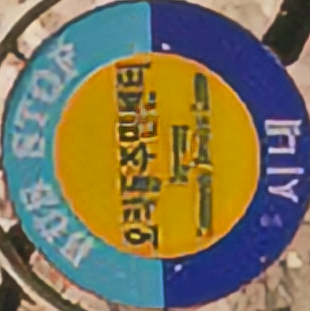
\includegraphics[width=\linewidth]{imgs/DASR_23.83_0.7483_Canon_020.png}
%             \caption{4} 
%         \end{subfigure}

%         \bigskip % some vertical space between subfigures a/b and c/d...
%         \begin{subfigure}{0.22\textwidth}
%             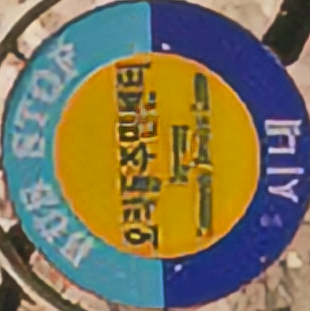
\includegraphics[width=\linewidth]{imgs/DASR_23.83_0.7483_Canon_020.png}
%             \caption{5} 
%         \end{subfigure}
%         \hfill
%         \begin{subfigure}{0.22\textwidth}
%             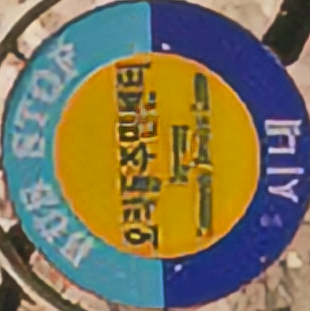
\includegraphics[width=\linewidth]{imgs/DASR_23.83_0.7483_Canon_020.png}
%             \caption{6} 
%         \end{subfigure}
%     \end{minipage}
    
    
% \end{figure}

\begin{figure}[htbp]
    \captionsetup[subfigure]{labelformat=empty} 
    \begin{subfigure}{0.3\textwidth}
        
\includegraphics[width=\linewidth]{imgs/GT_Canon_001.png}
        \caption{GT PSNR/SSIM} 
    \end{subfigure}
    \hfill
    \begin{subfigure}{0.3\textwidth}
        
\includegraphics[width=\linewidth]{imgs/STESRGAN_23.56_0.7960_Canon_001.png}
        \caption{ESRGAN 23.56/0.7960} 
    \end{subfigure}
    \hfill
    \begin{subfigure}{0.3\textwidth}
        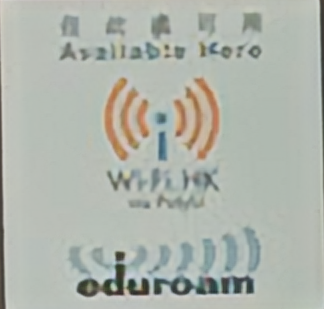
\includegraphics[width=\linewidth]{imgs/DASR_25.37_0.8651_Canon_001.png}
        \caption{DASR 25.37/0.8651} 
    \end{subfigure}
    \begin{subfigure}{0.3\textwidth}
        
\includegraphics[width=\linewidth]{imgs/LR_Canon_001.png}
        \caption{LR} 
    \end{subfigure}
    \hfill
    \begin{subfigure}{0.3\textwidth}
        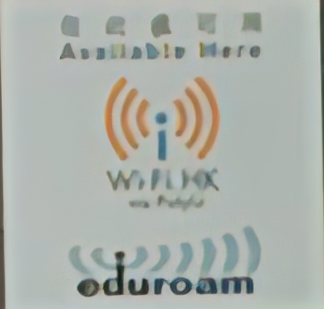
\includegraphics[width=\linewidth]{imgs/USR_DU_24.97_0.8570_Canon_001.png}
        \caption{USR-DU 24.97/0.8570} 
    \end{subfigure}
    \hfill
    \begin{subfigure}{0.3\textwidth}
        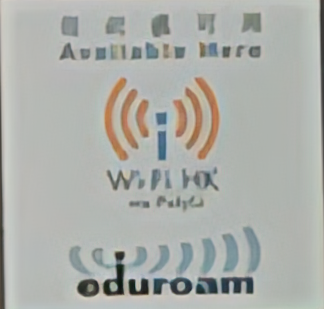
\includegraphics[width=\linewidth]{imgs/UBSR_DU_25.23_0.8749_Canon_001.png}
        \caption{UBSR-DU \textbf{25.23}/\textbf{0.8749}} 
    \end{subfigure}
    \caption{Canon\_001上的超分视觉效果对比}
    \label{fig:Canon001}
\end{figure}


\begin{figure}[htbp]
    \captionsetup[subfigure]{labelformat=empty} 
    \begin{subfigure}{0.3\textwidth}
        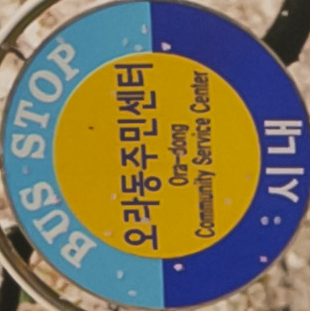
\includegraphics[width=\linewidth]{imgs/GT_Canon_020.png}
        \caption{GT} 
    \end{subfigure}
    \hfill
    \begin{subfigure}{0.3\textwidth}
        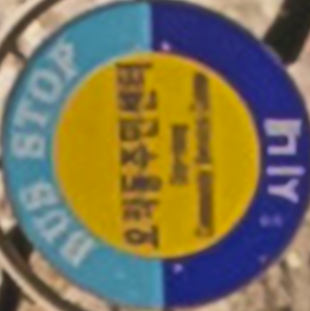
\includegraphics[width=\linewidth]{imgs/STESRGAN_23.65_0.7140_Canon_020.png}
        \caption{ESRGAN 23.65/0.7140} 
    \end{subfigure}
    \hfill
    \begin{subfigure}{0.3\textwidth}
        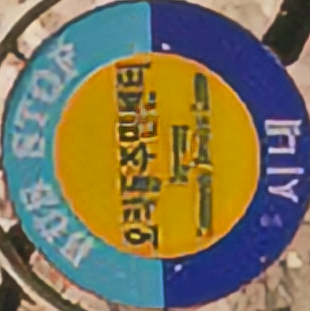
\includegraphics[width=\linewidth]{imgs/DASR_23.83_0.7483_Canon_020.png}
        \caption{DASR 23.83/0.7483} 
    \end{subfigure}
    \begin{subfigure}{0.3\textwidth}
        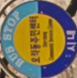
\includegraphics[width=\linewidth]{imgs/LR_Canon_020.png}
        \caption{LR} 
    \end{subfigure}
    \hfill
    \begin{subfigure}{0.3\textwidth}
        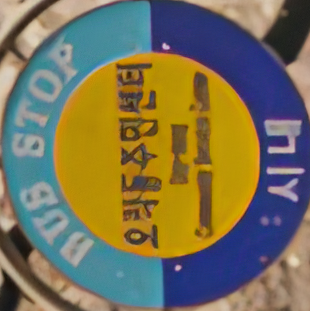
\includegraphics[width=\linewidth]{imgs/USR_DU_25.23_0.7589_Canon_020.png}
        \caption{USR-DU \textbf{25.23}/0.7589} 
    \end{subfigure}
    \hfill
    \begin{subfigure}{0.3\textwidth}
        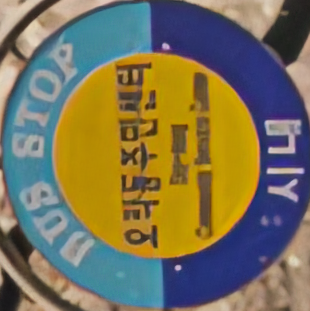
\includegraphics[width=\linewidth]{imgs/UBSR_DU_25.22_0.7819_Canon_020.png}
        \caption{UBSR-DU 25.22/\textbf{0.7819}} 
    \end{subfigure}
    \caption{Canon\_020上的超分视觉效果对比}
    \label{fig:Canon020}
\end{figure}


\begin{figure}[htbp]
    \captionsetup[subfigure]{labelformat=empty} 
    \begin{subfigure}{0.3\textwidth}
        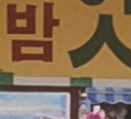
\includegraphics[width=\linewidth]{imgs/GT_Canon_033.png}
        \caption{GT} 
    \end{subfigure}
    \hfill
    \begin{subfigure}{0.3\textwidth}
        
\includegraphics[width=\linewidth]{imgs/STESRGAN_24.29_0.6954_Canon_033.png}
        \caption{ESRGAN 24.29/0.6954} 
    \end{subfigure}
    \hfill
    \begin{subfigure}{0.3\textwidth}
        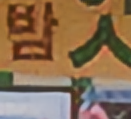
\includegraphics[width=\linewidth]{imgs/DASR_25.36_0.7601_Canon_033.png}
        \caption{DASR 25.36/0.7601} 
    \end{subfigure}
    \begin{subfigure}{0.3\textwidth}
        
\includegraphics[width=\linewidth]{imgs/LR_Canon_033.png}
        \caption{LR} 
    \end{subfigure}
    \hfill
    \begin{subfigure}{0.3\textwidth}
        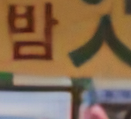
\includegraphics[width=\linewidth]{imgs/USR_DU_25.43_0.7440_Canon_033.png}
        \caption{USR-DU 25.43/0.7440} 
    \end{subfigure}
    \hfill
    \begin{subfigure}{0.3\textwidth}
        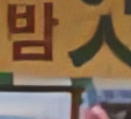
\includegraphics[width=\linewidth]{imgs/UBSR_DU_26.29_0.8093_Canon_033.png}
        \caption{UBSR-DU \textbf{26.29}/\textbf{0.8093}} 
    \end{subfigure}
    \caption{Canon\_033上的超分视觉效果对比}
    \label{fig:Canon033}
\end{figure}



\section{消融实验}
为了进一步验证我们所提出的方法的有效性和必要性,我们对模糊核估计模型的选择、模糊信息融入、数据集追加等方面进行了充分的消融实验。表\ref{tab:ablation}中展现了消融实验的结果。
% \begin{table}[htbp]
%     \begin{tabular}{c|cc|cc}
%         \toprule  
%           & 模糊核估计算法 & 模糊信息 & 数据集追加 & PSNR$\uparrow$  &  SSIM$\uparrow$ \\
%         \midrule
%         0 & $\xmark$ & & & 26.56 & 0.7736 \\
%         1(待定) & KULNet & $\cmark$ & $\cmark$ & 26.50 & 0.7630 \\[-1.5ex]\hline\noalign{\vspace{\dimexpr 1.87ex-\doublerulesep}}
%         2 & UFPNet & $\cmark$ & $\cmark$ & 8 & 9 \\
%         3 & MANet & $\cmark$ & & 26.42 & 0.7749 \\
%         4 & $\xmark$ & & $\cmark$ & 26.59 & 0.7662 \\
%         5 & MANet & $\cmark$ & $\cmark$ & \textbf{26.63} & \textbf{0.7748} \\
%         \bottomrule
%     \end{tabular}
%     \caption{消融实验}
%     \label{tab:ablation}
% \end{table}
\begin{table}[htbp]
    \centering
    \caption{消融实验}
    \label{tab:ablation}
    \begin{tblr}{
        colspec={cccccc},
        hline{1,8} = {1pt,solid},
        hline{2} = {0.5pt,solid},
        vline{2,3,5} = {0.5pt,solid}
    }
        & 模糊核估计算法 & 模糊信息 & 数据集追加 & PSNR$\uparrow$  &  SSIM$\uparrow$ \\
        0 & \xmark & & & 26.56 & 0.7736 \\
        1 & KULNet & \cmark & \cmark & 26.50 & \textbf{0.7751} \\
        2 & UFPNet & \cmark & \cmark &  &  \\
        3 & MANet & \cmark & & 26.42 & 0.7749 \\ 
        4 & \xmark & & \cmark & 26.59 & 0.7662 \\
        5 & MANet & \cmark & \cmark & \textbf{26.63} & 0.7748 \\
    \end{tblr}
\end{table}

\noindent\textbf{模糊核估计模型的选择}\ \ 比较第0、1、3项,其中1、3项中仅有模糊核估计部分发生了变化。可发现基于KULNet核估计的模型虽然SSIM高于USR-DU,但PSNR低于USR-DU,不能说明其整体优于USR-DU。而基于MANet核估计的模型则在两项指标上均优于USR-DU。

\noindent\textbf{模糊信息融合和额外数据集共同使用的必要性}\ \ 比较0和3两项,其中0为USR-DU原始模型,3中加入了模糊信息融合部分。第3项的SSIM较第0项有所提升,但PSNR有所下降。比较0和4两项,二者区别仅在于第4项的SRN部分额外使用了RealSR-Nikon训练集高分辨率图像作为训练集的一部分,可以发现第4项的PSNR较第0项有所提升,但SSIM有所下降。对比0,3,4,5项,可以证明只有模糊信息融合和额外数据集二者共同使用时才能使PSNR与SSIM均有明显的提升。

综上所述,选择UFPNet作为模糊核估计部分,为DSN的参考图像融合入模糊信息,并在训练SRN过程中额外使用RealSR-Nikon训练集高分辨率图像作为训练集的一部分是必要且有效的措施。

